\documentclass[11pt,addpoints,letterpaper]{exam}
\usepackage{amsmath,tcolorbox,mdframed,xcolor}
\usepackage[top=0.75in, bottom=0.85in, left=1in, right=1in]{geometry} % Adjust margins

\usepackage{siunitx}
\usepackage{nccmath}
\usepackage{physics}
\usepackage{tikz}
\usepackage{multicol}
\usepackage{xfrac}
\usepackage{wrapfig}

\usepackage{float}


\noprintanswers


% Define variables
\newcommand{\instructor}{Mr. Rodriguez}
\newcommand{\coursename}{Conceptual Physics A}
\newcommand{\term}{Fall}
\newcommand{\courseyear}{2024} % Renamed \year to \courseyear to avoid conflict
\newcommand{\instructions}{}
\newcommand{\worksheetname}{Final Exam}
\newcommand{\qsp}{\vspace{5cm}}
\newcommand{\qspp}{\vspace{2.5cm}}
\newcommand{\qsppp}{\vspace{0.5cm}}

\tcbset{
    myboxstyle/.style={
        colback=white,        % Background color
        colframe=black,       % Border color
        boxrule=0.5pt,        % Border thickness
        arc=5mm,              % Rounding radius
        boxsep=2mm,           % Padding around text
        left=4pt, right=4pt,  % Inner padding on left and right
    }
}
\newcommand{\equationbox}[2]{
\begin{center}
\begin{tcolorbox}[colframe=black!60, colback=white, arc=5mm, boxrule=0.75pt, title=#1]
% \vspace{-0.2in} % Tightens the space between the title and content
\begin{flushleft}
\begin{align*}
#2
\end{align*}
\end{flushleft}
\end{tcolorbox}
\end{center}
}
\newcommand{\equationboxx}[2]{
\begin{center}
\begin{tcolorbox}[colframe=black!60, colback=white, arc=5mm, boxrule=0.75pt, title=#1]
\begin{flushleft}
#2
\end{flushleft}
\end{tcolorbox}
\end{center}
}
\newcommand{\instructionbox}[1]{\begin{center}\fbox{\fbox{{\centering #1}}}\end{center}}

\newcommand{\learningStandard}[1]{
    \small
    \tcbox[colback=gray!10, colframe=black, boxrule=0.5mm, sharp corners=southwest]{
        \textbf{#1} \hspace{0.5cm} % Spacing between title and vertical rule
        \textcolor{gray}{\vrule height 10pt width 0.3pt}\hspace{0.5cm} % Lighter and thinner vertical rule
        \textbf{Score:} \rule{1.5cm}{0.5pt} /10
    }
}

\newtcolorbox{learningStandardBox}[2]{%
    title={Learning Standard #1}, % Title with manual input for the standard number
    fonttitle=\bfseries\small,  % Title font style
    colback=gray!15, % Background color for main content
    colframe=black, % Frame color
    coltitle=black!80, % Font color for title
    colbacktitle=gray!60, % Background color for title
    boxrule=0.5mm, % Border thickness
    sharp corners=south, % Rounded top corners only
    width=\textwidth, % Full text width
    halign=center, % Center-align content
    top=10pt, % Adds extra space at the top to move content down
}
\newcommand{\standardBox}[2]{%
    \begin{learningStandardBox}{#1}{#2} % Passes number and name as arguments
        \begin{minipage}[t]{0.5\textwidth} % Left section for standard name
            \textit{#2} % Italicized name of the standard
        \end{minipage}%
        \hfill
        \begin{minipage}[t]{0.25\textwidth} % Middle section for score
            \textbf{Score:} \rule{1.5cm}{0.5pt} /10
        \end{minipage}%
        \hfill
        \begin{minipage}[t]{0.2\textwidth} % Right section for grade
            \textbf{Grade:} \phantom{1.2cm}
        \end{minipage}
    \end{learningStandardBox}
}
%%%%%%%%%%%%%%%%%%%%%% BEGIN DOCUMENT %%%%%%%%%%%%%%%%%%%%%%%%%%%%%%%%%%%%%%%
\begin{document}

% Place name, section, and instructor details at the top left
\vspace*{-0.2in} % Adjust this to control vertical spacing from the top of the page
\noindent
\makebox[0.7\textwidth][l]{Name:\enspace\hrulefill} \hfill \makebox[0.3\textwidth]{ Period:\enspace\hrulefill} \\[1cm]
\noindent
\makebox[0.7\textwidth][l]{Instructor: \enspace\texttt{\instructor}}\hfill \hspace*{0pt}\hfill{Total Score:\underline{\hspace{2cm}}/\numpoints}
\vspace{0.5in} % Space before the title


% Manually add the title without using \maketitle
\begin{centering}
\noindent\textbf{\Large \worksheetname} \\[0.1in]
\noindent\texttt{\coursename} \\
\noindent\textit{\term\ \courseyear} \\
\end{centering}

\vspace{0.2in}

% Special Instructions
% \begin{center}
% \fbox{\fbox{\parbox{5.5in}{\centering
% \instructions}}}
% \end{center}


% Relevant Equations box with no extra space and left-aligned equations


%%%%%%%%%%%%%%%%%%%%%%%%%%%%%%%%%%%%%%%%%%% LS 1 %%%%%%%%%%%%%%%%%%%%%%%%%%%%%%%%%%%%%%
% \section*{\small \tcbox{Learning Standard 3.1: The Law of Conservation of Energy}}
% \section*{\learningStandard{Learning Standard 3.1: The Law of Conservation of Energy}}
\standardBox{3.1}{The Law of Conservation of Energy}

\instructionbox{\emph{Multiple Choice}: Circle \textbf{one} option per question.}

\begin{questions}

\question[2] Which of the following statements best describes the law of conservation of energy? 
\qsppp
\begin{choices}
\choice Energy can be created or destroyed, but it cannot change from one form to another.
\choice Energy can be transferred or transformed but is always lost in the process.
\CorrectChoice Energy cannot be created or destroyed; it can only change from one form to another.
\choice Energy can only be conserved in closed systems, and is always constant in open systems.
\end{choices}
\qsppp

\question[2] What are the SI (metric) units of energy?
\qsppp
\begin{choices}
\choice Newtons (N)
\choice kilograms (kg)
\CorrectChoice Joules (J)
\choice meters per second (m/s)
\end{choices}
\qsppp


\pagebreak
\instructionbox{\emph{Fill in the Blank}: For each blank space, choose \textbf{one} item from the word bank below.}

\equationboxx{Word Bank}{
\begin{multicols}{2}
    \begin{itemize}
    \item Chemical
    \item Electrical
    \item Elastic
    \item Gravitational Potential
    \item Kinetic
    \item Light
    \item Sound
    \item Thermal
    \end{itemize}
\end{multicols}
}
\question[3] Use the word bank above identify which types of energy are converted into which other types of energy by each machine. Some words may be used more than once; others may not end up used at all. 
\begin{parts}
\qsppp
\part A \textbf{loudspeaker} converts \fillin[electrical][3cm] energy into \fillin[sound][3cm] energy.
\qsppp
\part A \textbf{solar panel} converts \fillin[solar][3cm] energy into \fillin[electric][3cm] energy.
\qsppp
\part A \textbf{car engine} converts \fillin[chemical][3cm] energy into \fillin[kinetic][3cm] energy.
\qsppp
\part A \textbf{flashlight} converts \fillin[chemical][3cm] energy into \fillin[light][3cm] energy.
\qsppp
\part A \textbf{slingshot} converts \fillin[elastic][3cm] energy into \fillin[kinetic][3cm] energy.
\qsppp
\part A \textbf{hydroelectric turbine generator} converts \fillin[gravitational potential][3cm] energy into \fillin[electrical][3cm] energy. 
\end{parts}
\instructionbox{\emph{Free Response}: Answers must be in \textbf{complete sentences} to receive full credit.}
\question[3] Use your knowledge of the law of conservation of energy to explain how \emph{all} energy on Earth actually came from the Sun at one point or another. Make sure to include the following terms in your argument: \emph{solar, plants, animals, chemical energy, humans, fossil fuels}. 


\pagebreak

\standardBox{3.2}{Problem Solving via Conservation of Energy}

\question[10] Tony Hawk is skating on a flat, horizontal surface towards a circular loop, like the one shown in the figure below:
\begin{figure}[H]
    \centering
    % \vspace{0.2cm} % Add vertical space above the image
   \scalebox{-1}[1]{ 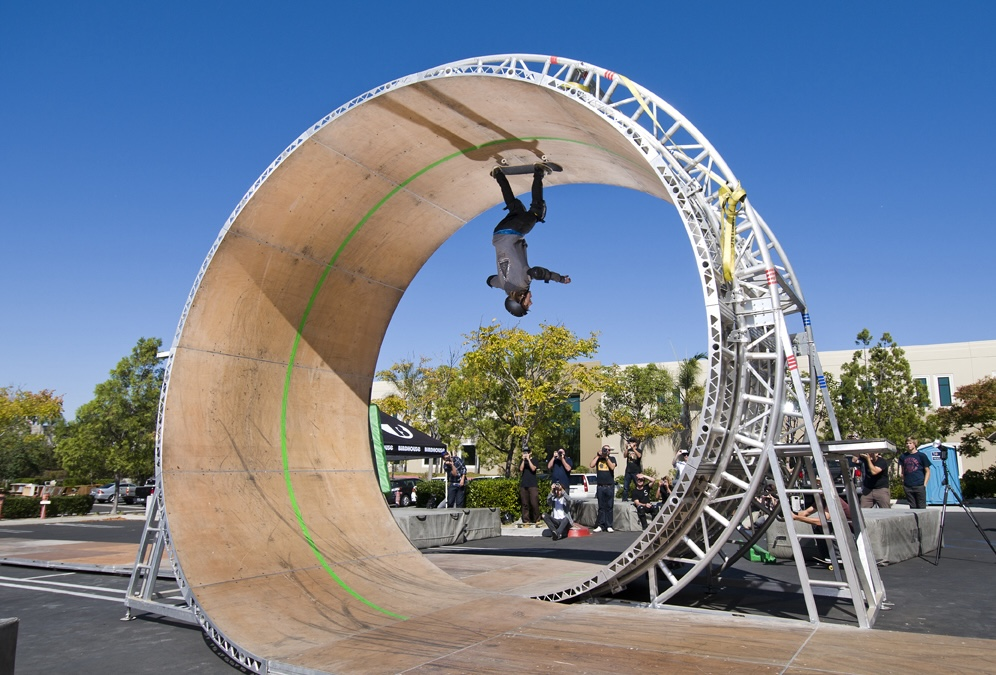
\includegraphics[width=0.45\textwidth]{loop.jpg}} % Specify image width and file name
    % \vspace{0.2cm} % Add vertical space below the image
\end{figure}

Conservation of energy tells us that the faster Tony is traveling on his skateboard before approaching the loop, the higher he will climb along the loop.
Tony wants to find the minimum speed he needs to successfully complete a full circular loop without falling back down. Assume the radius of the loop is $r=\SI{5}{m}$. What is the \emph{minimum} velocity \textbf{v} that Tony must have at the bottom of the loop to complete the full circle? Assume no friction or air resistance. 

\pagebreak
\standardBox{3.3}{Power and Generators}
\equationbox{Relevant Equations}
{
PE &= mgh & & \text{(Potential Energy)}\\
P &= \tfrac{\Delta E}{\Delta t} = \tfrac{\text{(change in energy)}}{\text{(change in time)}} & &\text{(Power)}
}
% Yosemite Falls, one of the tallest waterfalls in North America, has a total height of approximately \SI{740}{m}. During peak flow in spring, about \SI{50000}{kg} of water flows over the falls every second. Suppose engineers set up a hydroelectric turbine at the base of the falls to capture the energy from the falling water. 
% \begin{figure}[H]
%     \centering
%     % \vspace{0.2cm} % Add vertical space above the image
%    \scalebox{-1}[1]{ 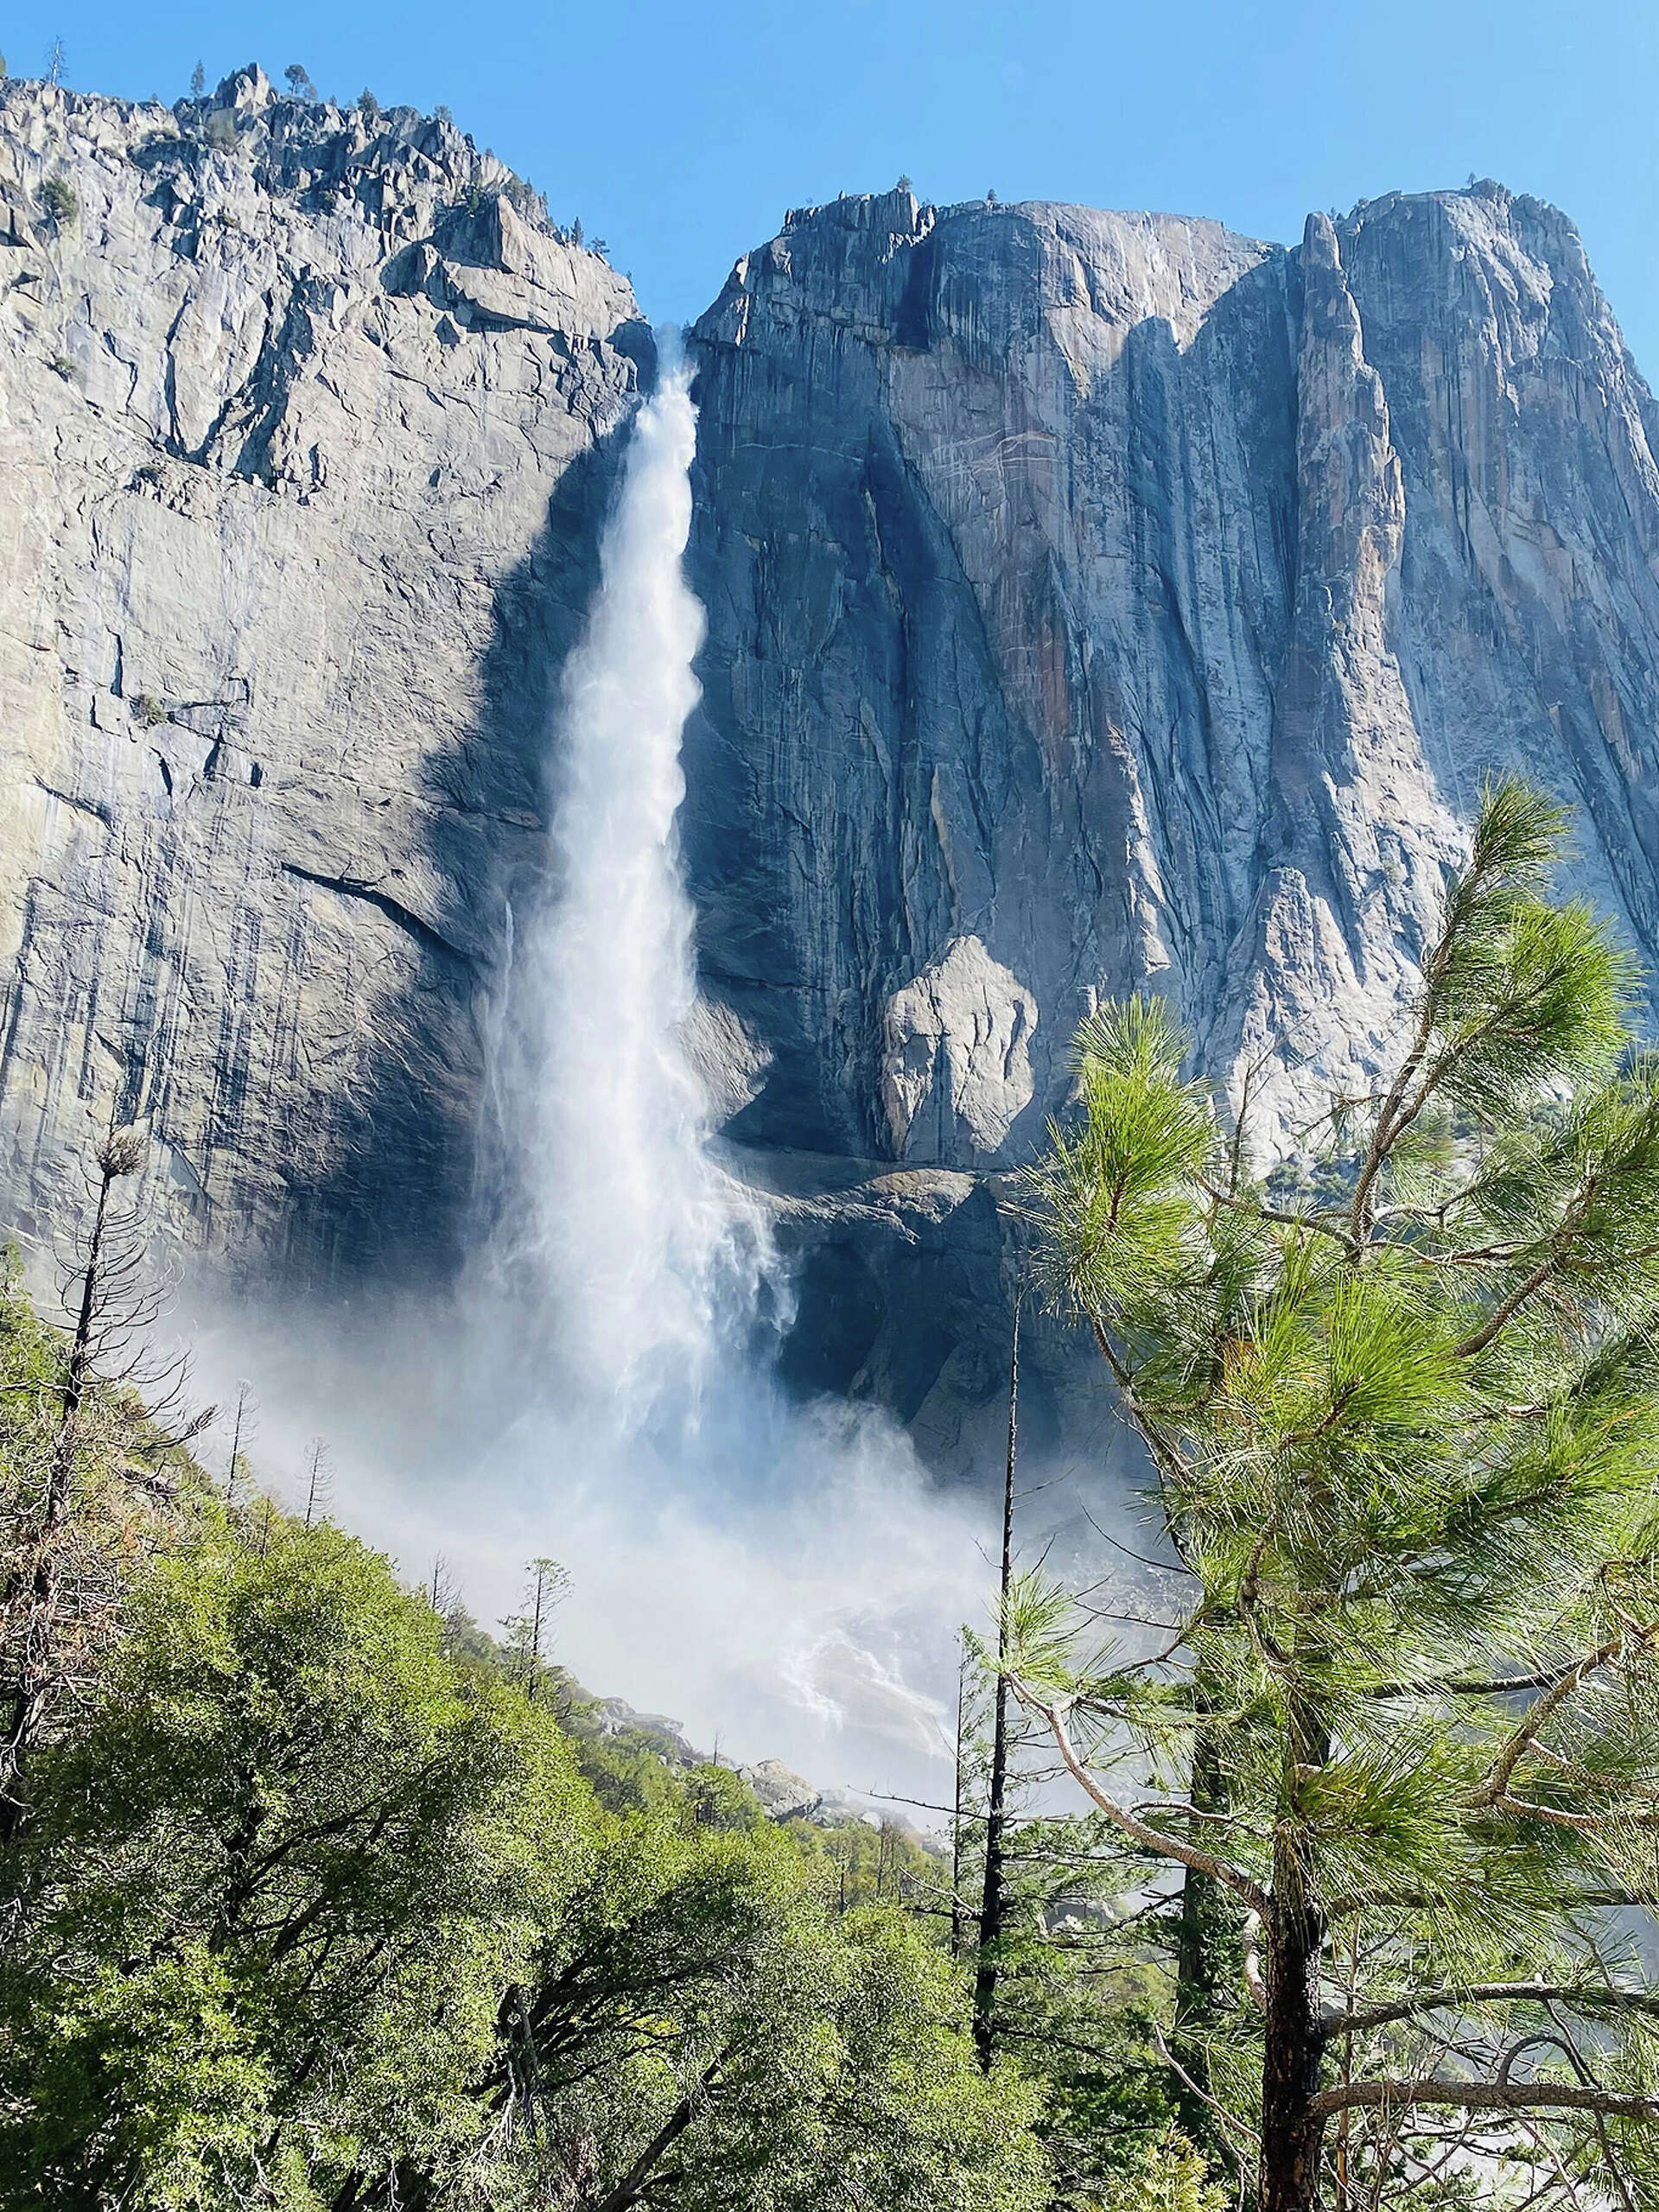
\includegraphics[width=0.45\textwidth]{yosemite.jpg}} % Specify image width and file name
%     % \vspace{0.2cm} % Add vertical space below the image
% \end{figure}
\noindent
\begin{minipage}{0.3\textwidth}
    \centering
    \fbox{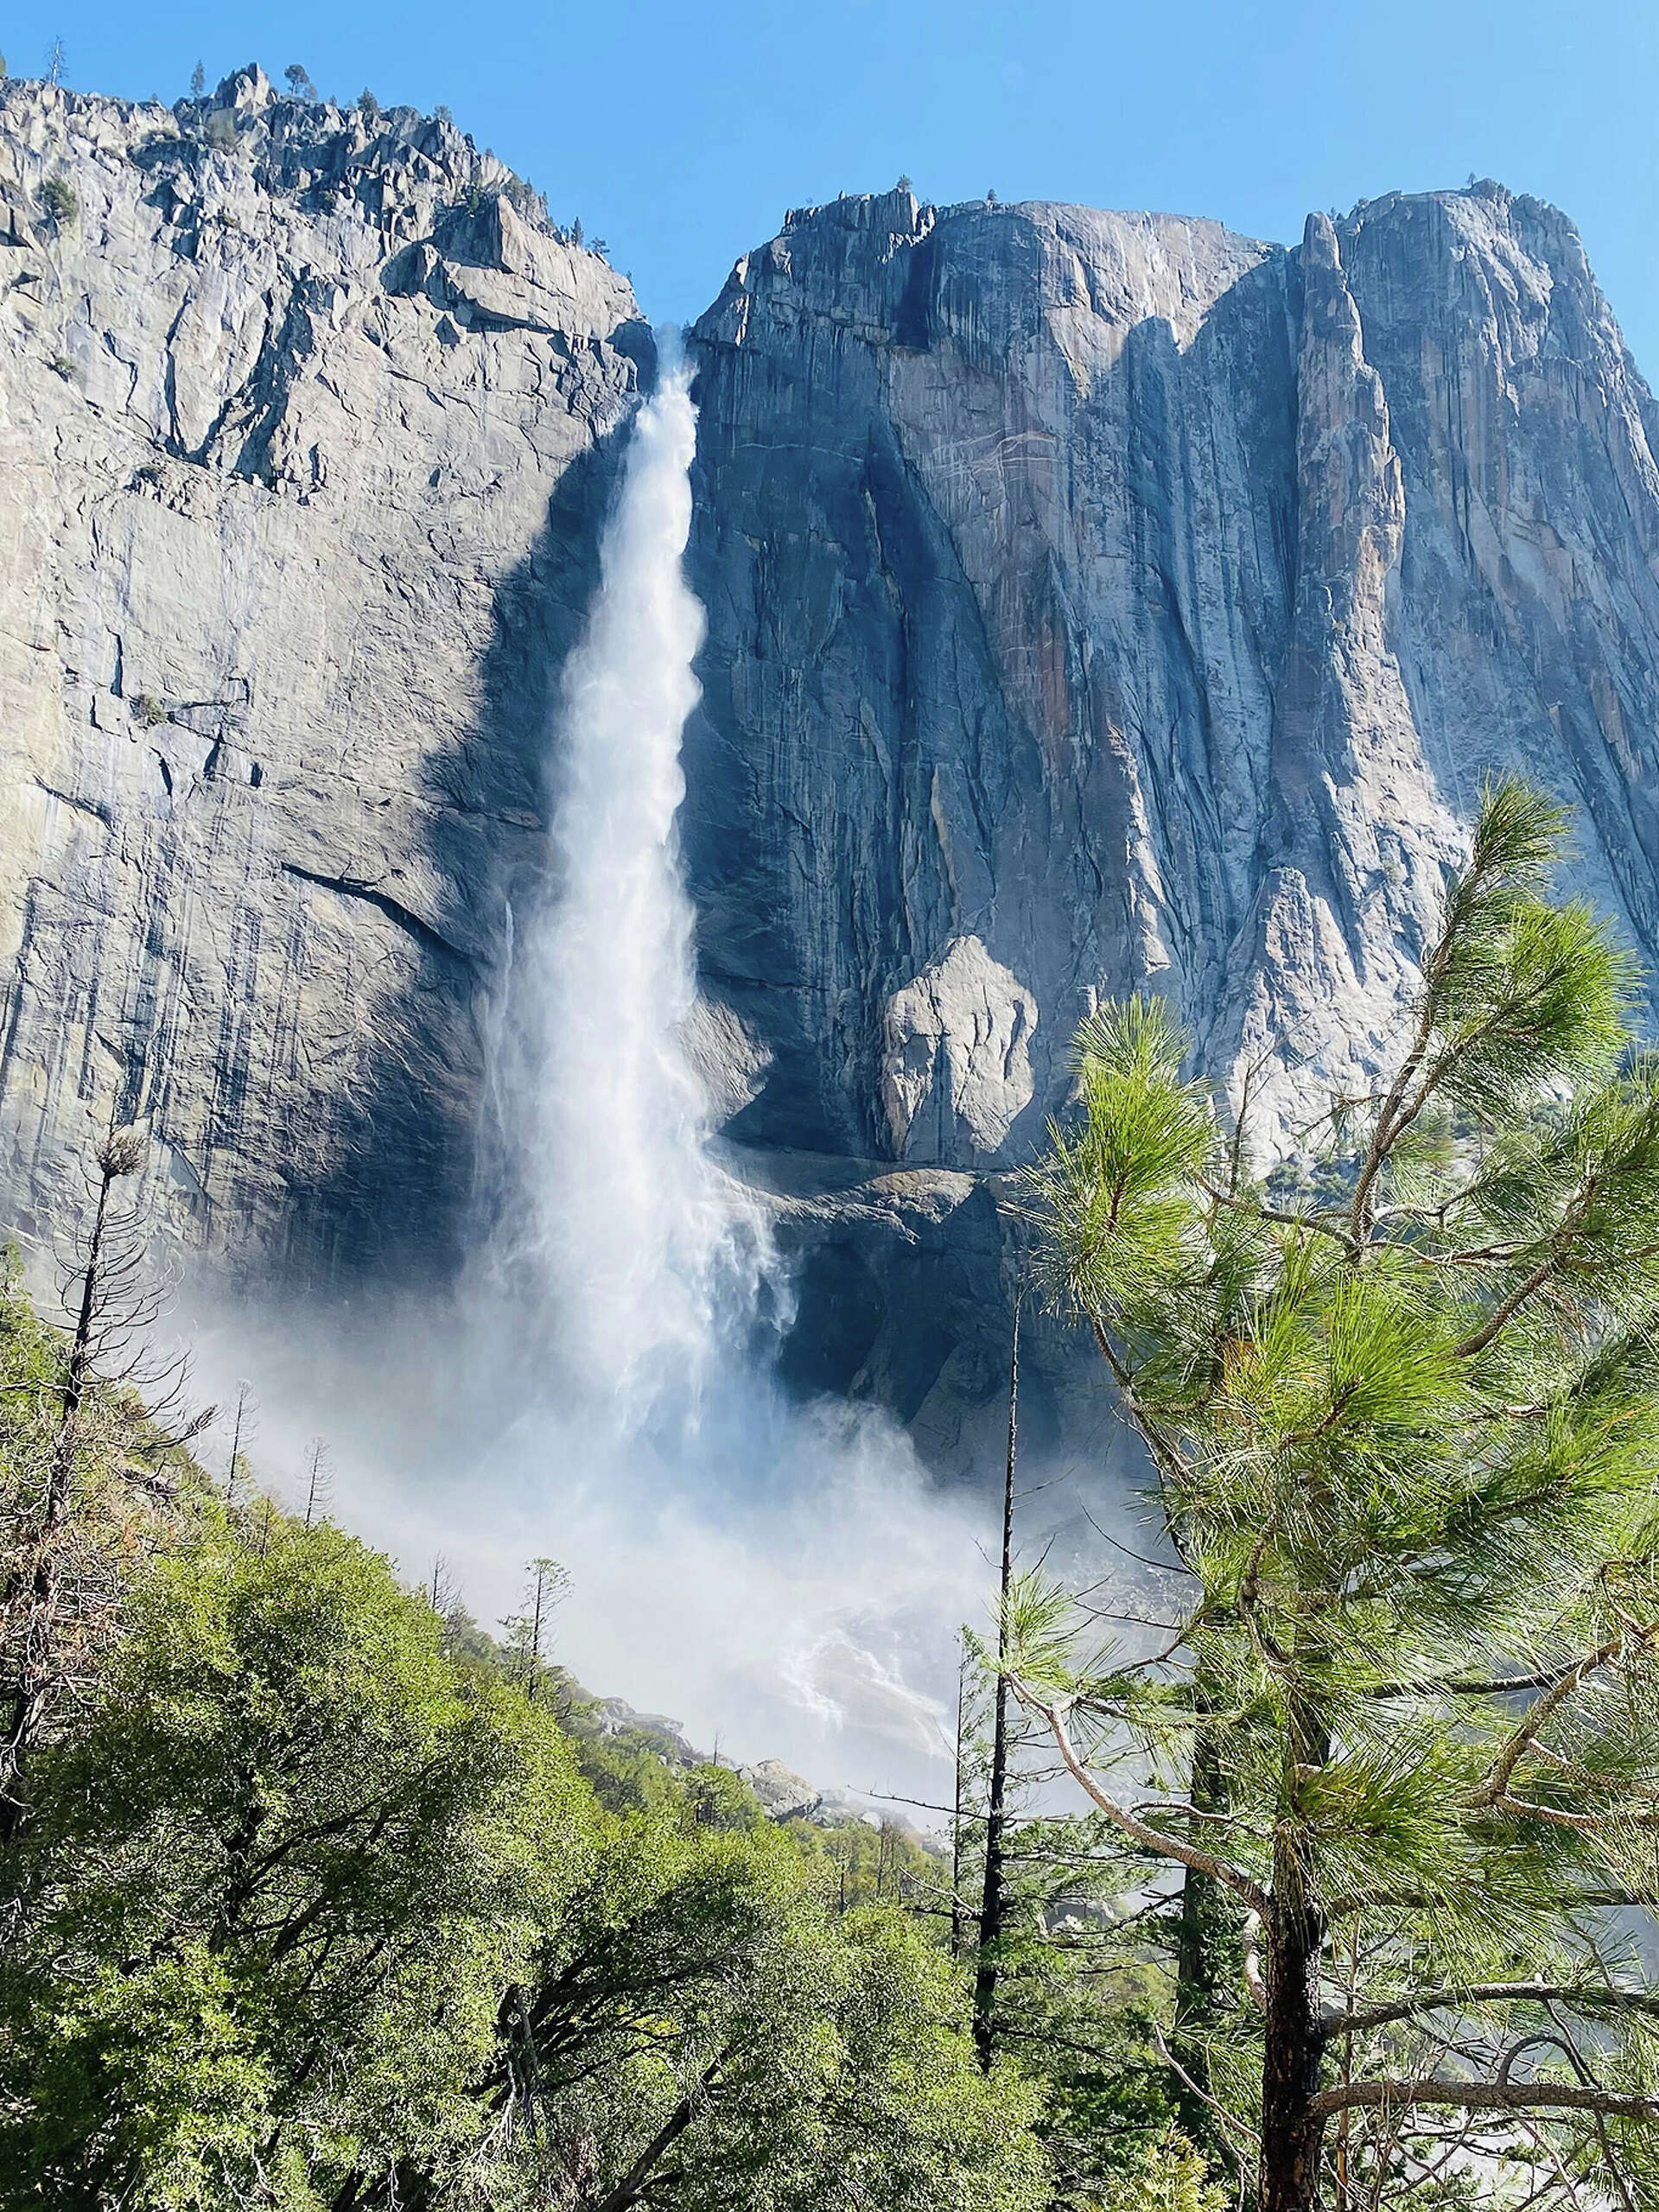
\includegraphics[width=0.7\textwidth]{yosemite.jpg}} % Flipped image, adjust width as needed
\end{minipage}
\begin{minipage}{0.7\textwidth}
    Yosemite Falls, one of the tallest waterfalls in North America, has a total height of approximately \SI{740}{m}. During peak flow in spring, about \SI{50000}{kg} of water flows over the falls every second. Suppose engineers set up a hydroelectric turbine at the base of the falls to capture the energy from the falling water.
\end{minipage}%

\vspace{0.5cm}
\question[2] What are the SI (metric) units of power?
\vspace{2.5cm}
\question[3] Calculate the gravitational potential energy of the water that falls from the height of Yosemite Falls in one second. 
\vspace{2.5cm}
\question[3] Calculate the theoretical power generated by the water flow. 
\vspace{2.5cm}
\question[2] How many \SI{40}{W} light bulbs could be powered by this hydroelectric turbine?

\pagebreak
\standardBox{3.4}{Energy and Automobile Safety}
\equationbox{Relevant Equations}
{
KE &= \tfrac{1}{2}mv^2 & &\text{(Kinetic Energy)}\\
W &= Fd & & \text{(Work)}
}
\question[3] A car with a mass of \SI{1200}{kg} is traveling at $v=\SI{12.5}{m/s}$ (about 45 km/h). The driver applies the brakes, and the car comes to a stop due to the friction between the tires and the road. 

\begin{parts}
\part Calculate the initial kinetic energy of the car. 
\vspace{2cm}
\part If the brakes apply a constant frictional force of 6,000 N, how far does the car travel before coming to a complete stop?
\end{parts}
\vspace{2cm}
\question[2] If the car was going twice as fast ($v=\SI{25}{m/s}$, which is about 90 km/h), by what factor would the kinetic energy increase? 
\vspace{2cm}

\question[3] At this doubled speed, how much farther would the car travel while applying the brakes to come to a stop? 
\qspp
\question[2] Based on your results, explain the relationship between the car's speed and the potential severity of a crash.

\end{questions}


\end{document}
